%% A simple template for a lab or course report using the Hagenberg setup
%% based on the standard LaTeX 'report' class
%%% äöüÄÖÜß  <-- no German umlauts here? Use an UTF-8 compatible editor!

%%% Magic comments for setting the correct parameters in compatible IDEs
% !TeX encoding = utf8
% !TeX program = pdflatex 
% !TeX spellcheck = en_US
% !BIB program = biber

\documentclass[english,notitlepage,smartquotes]{hgbreport}
% Valid options in [..]: 
%    Main language: 'german' (default), 'english'
%    Turn on smart quote handling: 'smartquotes'
%    APA bibliography style: 'apa'
%    Do not create a separate title page: 'notitlepage'
%%%-----------------------------------------------------------------------------

\RequirePackage[utf8]{inputenc} % Remove when using lualatex or xelatex!

\renewcommand{\chapter}[1]{} % Disable \chapter command
\graphicspath{{images/}}     % Location of images and graphics
\bibliography{references}    % Biblatex bibliography file (references.bib)
\ExecuteBibliographyOptions{backref=false} % No back references in bibliography

%%%-----------------------------------------------------------------------------
\setcounter{chapter}{1}	% <----- set to assignment number!
%%%-----------------------------------------------------------------------------

\author{Julian Emanuel Jany}                     % Your name
\title{Evaluation and identification of the optimization potential of modern demosaicing algorithms \\ % Name of the course
			 \textbf{Exposé}}
\date{\today}

%%%-----------------------------------------------------------------------------
\begin{document}
%%%-----------------------------------------------------------------------------
\maketitle
%%%-----------------------------------------------------------------------------

% \begin{abstract}\noindent
% This lab unit deals with various interesting problems \ldots (give a short
% summary of the specific topics addressed). If you decide to write your report in
% German, make sure to change the \verb!\documentclass! parameter from
% \texttt{english} to \texttt{german}.
% If you write in MS Word (and such), try to use a similar structure.
% \end{abstract}

%%%-----------------------------------------------------------------------------

\section{Motivation}

The majority of imaging devices utilize only a single image sensor, resulting in an inherently one-dimensional signal. 
To enable multi-spectral imaging, a \emph{Color Filter Array (CFA)} is placed on top of the sensor array. 
Typically, the CFA is implemented as a repeating pattern of three different filters. 
The most popular CFA is the \emph{Bayer CFA} (see Fig. \ref{fig:bayer_cfa}).

\begin{figure}[]
	\centering
	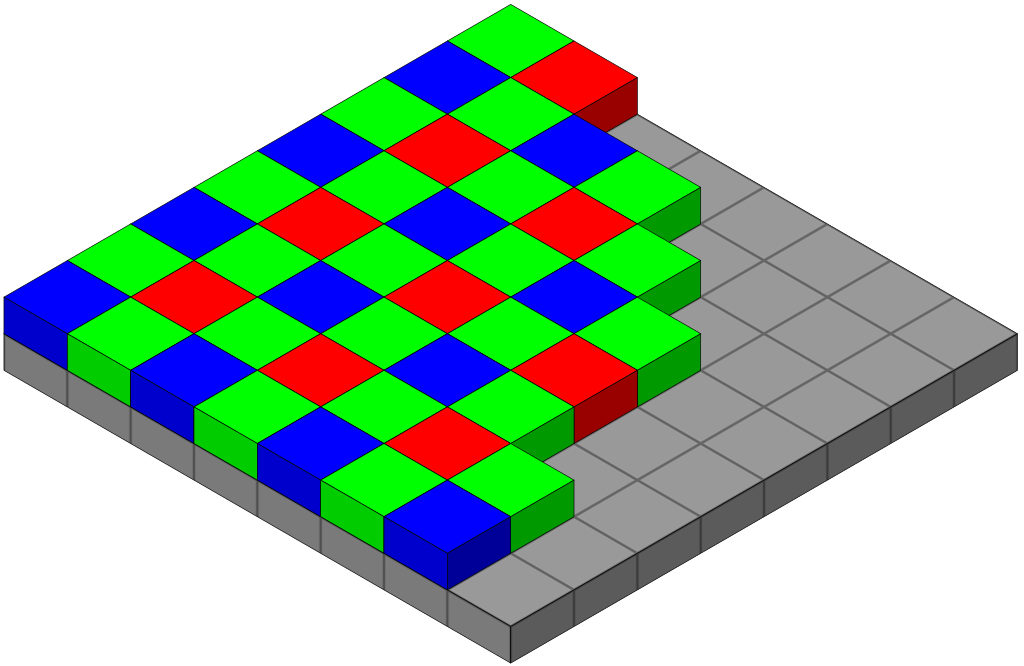
\includegraphics[width=0.3\textwidth]{bayer_pattern}
\caption{Image sensor array partially covered by a Bayer CFA. \cite{BayerCFA}}
\label{fig:bayer_cfa}
\end{figure}

Demosaicing is the process of reconstructing the two missing color channel signals for each sensel of the sensor to obtain a "full-color" image. 
This is usually one of the first stages of a digital imaging pipeline and significantly impacts the quality of the final image. 
Capturing high-quality, high-resolution images is of great interest to both research and industry. % Trinity of Pixel Enhancement: a Joint Solution for Demosaicking, Denoising and Super-Resolution

\section{Objectives} % "Ziele"

\subsection{Summary and Introduction}

The introduction of the master's thesis is intended to provide a detailed summary of related work and a comprehensive introduction to the state-of-the-art in demosaicing.

\subsection{Analysis}

The following chapter of the thesis represents a thorough analysis of several state-of-the-art demosaicing algorithms. 
Findings from this analysis are used to identify potential for improvement in specific aspects.

\noindent
Possible improvement aspects:

\begin{itemize}
	\item Runtime performance
	\item Memory footprint
	\item Efficiency
	\item Artifact reduction (e.g. moiré, false color)
	\item Quality metrics (e.g. CPSNR)
	\item Visual/perceptual quality
\end{itemize}

\subsection{Prototypes}

Based on this assessment, multiple prototypes are developed, and it is determined whether significant improvements in the targeted aspects are achievable. 
The prototypes are thoroughly analyzed and compared with their respective reference algorithm.

\section{Tasks}

\begin{itemize}
	\item Study of related work
	\item Summary of related work and state-of-the-art algorithms
	\item Analysis of state-of-the-art algorithms
	\item Identification of aspects for improvement
	\item Implementation of prototypes
	\item Testing / Benchmarking prototypes
	\item Documenting achieved improvements
\end{itemize}

\section{Research Questions}

\begin{itemize}
	\item Which aspects of modern demosaicing algorithms offer potential for improvement?
	\item Can demosaicing quality be improved without large increases in runtime or memory usage?
	\item Can runtime or memory usage be decreased without lowering the perceptual quality?
\end{itemize}

% Vorgehensweise

\section{Organizational Details}

The master thesis is written in English.
There is no intention to block the publication of the master thesis.

\section{Milestones}

\subsection{Table of Contents}

The table of contents is handed in by \textbf{January 20, 2023} at the latest.

\subsection{Sample Chapter}

The sample chapter is handed in by \textbf{March 17, 2023} at the latest.

\subsection{Bibliography}

The bibliography is handed in by \textbf{April 28, 2023} at the latest.

\subsection{Preliminary Thesis}

The preliminary thesis is handed in by \textbf{May 29, 2023} at the latest.

\subsection{Final Thesis}

The final thesis is handed in by \textbf{June 26, 2023} at the latest.

\section{Relevant Literature}

Mittal et al. (2013) \cite{Mittal2013} introduced a model for blind evaluation of image quality. 
Unlike the quality metrics commonly used to compare demosaicing algorithms -- such as the Color Peak Signal-to-Noise Ratio (CPSNR) \cite{Menon2011} -- the proposed Natural Image Quality Evaluator (NIQE) does not require full-color reference images. 
NIQE can be used to evaluate the demosaicing quality for full-resolution images for which no full-color reference image exists. 
This is the case for all photographs taken with consumer cameras, since the JPEG output of the camera or raw-processor itself inherently contains demosaicing artifacts.

Menon et al. (2011) \cite{Menon2011} provide a comprehensive overview of classical demosaicing approaches.

Gharbi et al. (2016) \cite{Gharbi2016} were the first to apply a data-driven approach to the demosaicing problem. 
They used convolutional neural networks trained on "real" images to restore the missing data. 
The proposed approach showed qualitative improvements over the state-of-the-art on various data sets. 
Additionally, they have shown that the traditional approach of separating demosaicing and denoising as sequential steps in the image processing pipeline is suboptimal.

Ronneberger et al. (2015) \cite{Ronneberger2015} proposed the U-Net for biomedical image segmentation. 
The network architecture has since produced excellent results in various different domains. 
An adapted U-Net is a promising candidate for one of the prototypes.

Kim et al. (2020) \cite{Kim2020} demonstrate an innovative demosaicing algorithm that builds on prior work in multiple fields. 
Their approach yields outstanding results for the challenging Quad Bayer CFA.

%%%-----------------------------------------------------------------------------
  
\section*{References}

\printbibliography[heading=noheader]

%%%-----------------------------------------------------------------------------
\end{document}
%%%-----------------------------------------------------------------------------
